%% 
%% Copyright 2019-2024 Elsevier Ltd
%% 
%% This file is part of the 'CAS Bundle'.
%% --------------------------------------
%% 
%% It may be distributed under the conditions of the LaTeX Project Public
%% License, either version 1.3c of this license or (at your option) any
%% later version.  The latest version of this license is in
%%    http://www.latex-project.org/lppl.txt
%% and version 1.3c or later is part of all distributions of LaTeX
%% version 1999/12/01 or later.
%% 
%% The list of all files belonging to the 'CAS Bundle' is
%% given in the file `manifest.txt'.
%% 
%% Template article for cas-sc documentclass for 
%% double column output.

\documentclass[a4paper,fleqn]{cas-sc}

% If the frontmatter runs over more than one page
% use the longmktitle option.

%\documentclass[a4paper,fleqn,longmktitle]{cas-sc}

%\usepackage[numbers]{natbib}
%\usepackage[authoryear]{natbib}
\usepackage[authoryear,longnamesfirst]{natbib}

%%%Author macros
\def\tsc#1{\csdef{#1}{\textsc{\lowercase{#1}}\xspace}}
\tsc{WGM}
\tsc{QE}
%%%

% Uncomment and use as if needed
%\newtheorem{theorem}{Theorem}
%\newtheorem{lemma}[theorem]{Lemma}
%\newdefinition{rmk}{Remark}
%\newproof{pf}{Proof}
%\newproof{pot}{Proof of Theorem \ref{thm}}

\begin{document}
\let\WriteBookmarks\relax
\def\floatpagepagefraction{1}
\def\textpagefraction{.001}

% Short title
\shorttitle{Learning dynamics as a heterogeneous cellular automaton}    

% Short author
\shortauthors{Sy et al.}  

% Main title of the paper
\title [mode = title]{Learning dynamics as a heterogeneous cellular automaton: comparing broadcast and nearest-neighbor interaction regimes in a classroom model}  

% Title footnote mark
% eg: \tnotemark[1]
% \tnotemark[1] 

% Title footnote 1.
% eg: \tnotetext[1]{Title footnote text}
% \tnotetext[1]{} 

% First author
%
% Options: Use if required
% eg: \author[1,3]{Author Name}[type=editor,
%       style=chinese,
%       auid=000,
%       bioid=1,
%       prefix=Sir,
%       orcid=0000-0000-0000-0000,
%       facebook=<facebook id>,
%       twitter=<twitter id>,
%       linkedin=<linkedin id>,
%       gplus=<gplus id>]

\author[1]{Clarence Ioakim T. Sy}
\credit{Software, Visualization, Writing - original draft}

\author[2]{Ranzivelle Marianne L. Roxas-Villanueva}
\credit{Conceptualization, Data curation, Resources, Supervision, Writing - review \& editing}

\author[1]{Johnrob Y. Bantang}
\cormark[1]
\ead{jybantang@up.edu.ph}
\credit{Conceptualization, Methodology, Formal analysis, Supervision, Writing - review \& editing}

\cortext[1]{Corresponding author}

\affiliation[1]{
    organization={National Institute of Physics, University of the Philippines Diliman},
    city={Quezon City},
    country={Philippines}}

\affiliation[2]{
    organization={Institute of Physics, University of the Philippines Los Ba\~{n}os},
    city={Laguna},
    country={Philippines}}

% For a title note without a number/mark
%\nonumnote{}

% Here goes the abstract
\begin{abstract}
  We present a probabilistic cellular automata (pCA) model to investigate the spatio-temporal learning dynamics of a classroom as a binary-state, heterogeneous agent system. Two interaction topologies are compared: a broadcast (mean-field-like) regime corresponding to traditional instruction (TI), and a nearest-neighbor coupling regime corresponding to peer instruction (PI). We characterize system behavior through the total relaxation time $t_{\rm max}$ as a function of class size $N$, mean agent learning rate $\lambda_0$, learning rate heterogeneity $\delta\lambda$, and spatial coupling strength $\rho_0$. In the broadcast regime, strong heterogeneity ($\delta\lambda \to 0.5$) produces a two-stage relaxation: a fast initial stage driven by high-$\lambda$ agents, followed by a slow residual stage governed by the low-$\lambda$ subpopulation. The nearest-neighbor regime is more robust to heterogeneity, exhibiting a more uniform relaxation curve with only a gradual shift in onset---a behavior attributable to percolation-driven spreading dynamics. The broadcast regime is favored for large $N$ and low $\delta\lambda$, while nearest-neighbor coupling tends to outperform for small $N$ and high $\delta\lambda$; however, the performance difference is notably larger in the latter regime than the former. We further analyze the fixed-point structure of the learning dynamics via a return map, from which class-level Hake gains are approximated. The nearest-neighbor regime yields a gain function consistent with existing theoretical predictions, while the broadcast regime yields an approximately constant gain. Results are compared against empirical classroom data, showing qualitative agreement.
\end{abstract}

% Use if graphical abstract is present
%\begin{graphicalabstract}
%\includegraphics{}
%\end{graphicalabstract}

% Research highlights
\begin{highlights}
\item pCA model of classroom learning under broadcast and nearest-neighbor topologies
\item Two-stage relaxation in heterogeneous broadcast systems; absent in local coupling
\item Local coupling is robust to heterogeneity through percolation-driven spreading
\item Return map yields analytic Hake gain expressions for both interaction regimes
\end{highlights}


% Keywords
% Each keyword is seperated by \sep
\begin{keywords}
cellular automata \sep complex systems \sep opinion dynamics \sep 
heterogeneous agents \sep percolation \sep learning dynamics
\end{keywords}

\maketitle

% Main text
\section{Introduction}\label{sec:intro}

Cellular automata (CA) models have become a well-established framework for studying the emergence of collective behavior in spatially extended systems of interacting agents~\citep{kari2005catheory, zaitsev2017generalized, louis2018probabilistic, Batac2009, arciaga2009experimental}.
Their discrete, lattice-based structure makes them particularly well-suited for capturing local interaction rules that give rise to complex macroscopic dynamics --- properties exploited across a broad range of applications from epidemic spreading~\citep{Beauchemin2005} to opinion formation and social dynamics~\citep{castellano2009statistical}.
A common thread across these systems is the interplay between local and global coupling: whether agents interact primarily with their immediate neighbors or receive information from a broadcast source shapes the relaxation behavior of the system in fundamentally different ways.
This distinction --- between nearest-neighbor and mean-field-like interaction topologies --- is generally understood to give rise to qualitatively different dynamical regimes across a variety of spatially extended systems.

A key variable in such systems is the degree of agent heterogeneity --- the spread in individual agent parameters such as coupling strength or response rate.
The degree of agent heterogeneity and local interaction environment have both been shown to significantly affect emergent collective dynamics in spatially explicit CA and agent-based models~\citep{lopez2014addressing, brown2006effects, jiao2011emergent}.
The spatial arrangement of agents and the reach of their interactions further shape these dynamics, as the neighborhood structure of the lattice directly governs the propagation pathways available to the system~\citep{dong2021influence, kari2005catheory}.
These considerations have been explored in the context of social systems, where CA-based models have demonstrated that interaction topology can be as significant as intrinsic agent parameters in determining system-level outcomes~\citep{bordogna2001theoretical, bordogna2003simulation, castellano2009statistical}.

The classroom provides a concrete and well-defined instantiation of such a heterogeneous agent system.
Students occupy fixed spatial positions on a lattice, interact with neighbors under rules governed by individual learning rates, and are subject to either a broadcast information source or local peer interaction.
Prior work by Bordogna and Albano~\citep{bordogna2001theoretical, bordogna2003simulation} demonstrated that CA-based models can capture essential features of classroom learning, including the influence of peer interaction and group structure on student outcomes.
The present work builds on this foundation by examining how the choice of interaction topology --- broadcast versus nearest-neighbor --- shapes collective relaxation dynamics in a heterogeneous CA classroom model.

We present a probabilistic cellular automata (pCA) model in which each agent is assigned a binary state and an individual learning rate $\lambda$, drawn from a two-level heterogeneous distribution parameterized by $\delta\lambda$.
Two interaction regimes are implemented and compared: a broadcast regime in which each agent updates independently based on a global source, and a nearest-neighbor regime in which updates depend on the states of adjacent lattice sites.
We characterize the collective dynamics through the total relaxation time $t_{\rm max}$ as a function of system size $N$, mean learning rate $\lambda_0$, heterogeneity $\delta\lambda$, and coupling strength $\rho_0$.
The effects of spatial configuration are also examined through a set of seating arrangements that determine the initial placement of learned agents in the nearest-neighbor regime, following prior empirical and computational work on the role of seating in classroom learning outcomes~\citep{roxas2010seating, monterola2009}.
We further validate our model against empirical classroom data by analyzing the fixed-point structure of the learning dynamics through a return map approach.
The return map is connected to the Hake gain~\citep{hake1998} --- a widely used measure of learning improvement between two successive assessments defined as
%%
\begin{equation}
    g \equiv (S_2 - S_1) / (1 - S_1)
\end{equation}
%%
where $S_1$ and $S_2$ are the scores of the first and second assessment respectively.
The Hake gain has been shown to follow characteristic functional forms that arise naturally from the assumptions of different theoretical models of the learning process~\citep{nitta2019mathematical, pritchard2008mathematical}, expressed through the recurrence relation
%%
\begin{equation}
    S_2 = S_1 + g(S_1) \cdot (1 - S_1)
\end{equation}
%%
where $g$ may in general be a function of $S_1$.
We show that the gain functions extracted from our simulation data via this return map are consistent with existing theoretical predictions~\citep{nitta2019mathematical, pritchard2008mathematical}, and we propose the return map as a practical method for empirically estimating class-level Hake gains from pre- and post-test data.

\section{Cellular Automata Method}\label{sec:methods}

We model classroom learning dynamics using a probabilistic cellular automata (pCA) model~\citep{SelfSPP}, a class of spatially extended dynamical systems in which discrete agents update their states stochastically according to local interaction rules~\citep{louis2018probabilistic, Fernandez2018}.
Each cell in the automaton represents an agent occupying a fixed position on a two-dimensional rectangular lattice --- as opposed to other lattice geometries such as hexagonal grids --- with agent interactions governed by the Moore neighborhood~\citep{kari2005catheory, zaitsev2017generalized}.
For a lattice of side length $L$, each agent is assigned a unique position $(i,j)$ with $i,j\in[1,L]$, giving a total population size $N=L^2$.
Agents at the edges and corners of the lattice have fewer neighbors, consistent with physical boundary conditions.

Each agent at position $(i,j)$ is assigned a binary state $s_{i,j}\in\{0,1\}$, representing two distinct levels of knowledge: \textit{unlearned} ($s_{i,j}=0$) and \textit{learned} ($s_{i,j}=1$).
Each agent is further assigned an individual learning rate $\lambda_{i,j}\in\mathcal{R}$, with $0<\lambda_{i,j}<1$, which governs the probability of transitioning from the unlearned to the learned state at each time step.
To introduce a heterogeneous agent population, we adopt a two-level distribution about a fixed mean $\lambda_0=0.5$, such that $\lambda_{i,j}=\lambda_0\pm\delta\lambda$.
The parameter $\delta\lambda\in[0.0, 0.4]$ serves as a tunable heterogeneity parameter, ranging from a fully homogeneous population ($\delta\lambda=0$) to a maximally heterogeneous one ($\delta\lambda=0.4$), with the constraint $0<\lambda_{i,j}<1$ bounding the accessible range.

At each time step $t\leftarrow(t+1)$, the state of each agent is updated according to a general algorithm (Fig.~\ref{fig:pCA-flowchart}) that encompasses both interaction regimes considered in this work.
\begin{figure}[htbp]
    \centering
    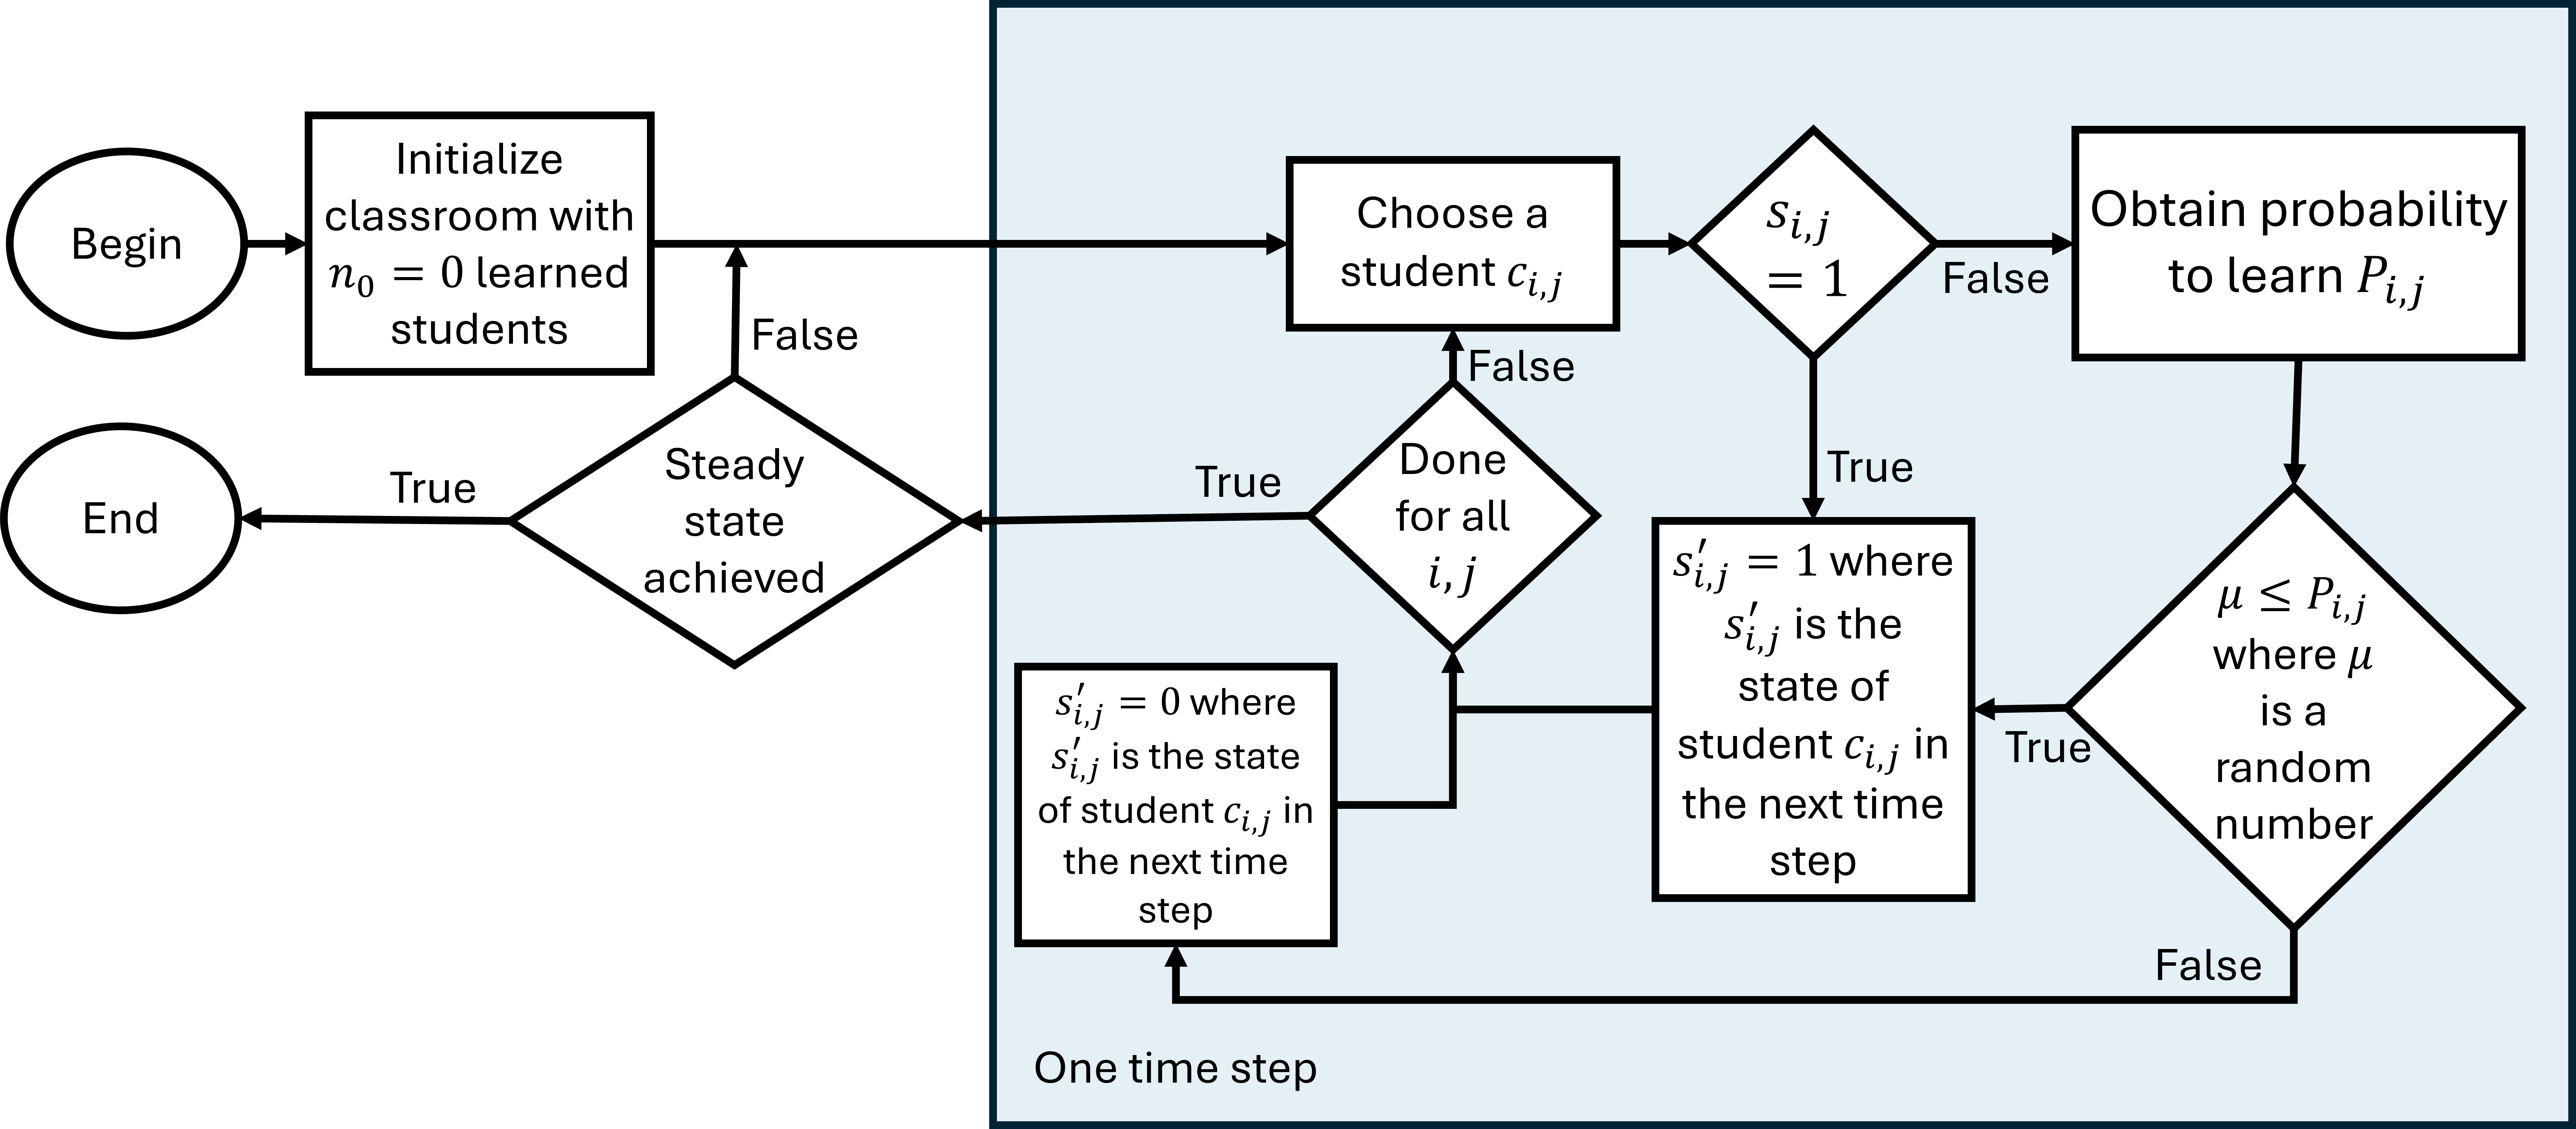
\includegraphics[width=\textwidth]{figs/2DBPCA Flowchart.png}
    \caption{
    Flowchart for the pCA algorithm used in this work.
    The broadcast (TI) and nearest-neighbor (PI) regimes differ in how the update probability $P_{i,j}$ is determined, as described in the text.
    }
    \label{fig:pCA-flowchart}
\end{figure}
The two regimes differ in how the update probability $P_{i,j}$ is determined, corresponding to the two modes of instruction being modeled.

For the broadcast regime (traditional instruction, TI), the update probability is given by
%%
\begin{equation}
\label{eq:TI-mode-probability}
    P_{i,j} = \lambda_{i,j}\;\rho_{\delta i,\delta j}
\end{equation}
%%
where $\rho_{\delta i,\delta j}\in[0,1]$ encodes the potential dependence of the learning efficiency on the relative position of the information source with respect to the agent~\citep{dong2021influence}.
In the broadcast regime, each agent receives information directly from a global source, analogous to a lecturer addressing the entire class simultaneously.
We simplify by fixing $\rho_{\delta i,\delta j}=\rho_0$ as a uniform, isotropic coupling strength, giving $P_{i,j}=\lambda_{i,j}\rho_0$.

For the nearest-neighbor regime (peer instruction, PI), the update probability additionally depends on the states of adjacent agents.
The compounded probability of learning from any learned neighbor is given by
%%
\begin{equation}
\label{eq:BPCA PI learning probability}
    P_{i,j} = 1 - \prod_{\forall \delta i, \delta j}{\left[1-(\lambda_{i,j}\;\rho_{\delta i, \delta j})(s_{i+\delta i, j+\delta j})\right]}
\end{equation}
%%
where the product runs over all neighbors of agent $(i,j)$, and $s_{i',j'}$ is the state of the neighboring agent at position $(i'=i+\delta i,\; j'=j+\delta j)$.
We again simplify by fixing $\rho_{\delta i,\delta j}=\rho_0$ for $|\delta i|\leq1$ and $|\delta j|\leq1$, and zero otherwise, corresponding to a Moore neighborhood with isotropic coupling~\citep{kari2005catheory, zaitsev2017generalized, louis2018probabilistic}.
Higher-order neighborhood interactions are possible but not considered here.

All broadcast regime simulations are initialized with all agents in the unlearned state, while nearest-neighbor regime simulations are initialized with four learned agents placed according to the chosen seating arrangement.
The total relaxation time $t_{\rm max}$ is defined as the number of iterations required for the system to reach steady state, which is considered achieved when either all agents have transitioned to the learned state, or when no transitions are recorded for 100 consecutive time steps.
The latter condition prevents prohibitively long waiting times for agents with very unfavorable combinations of learning rate, coupling strength, and neighborhood configuration.

The spatial configuration of initially learned agents in the nearest-neighbor regime is determined by the seating arrangement (SA), illustrated in Fig.~\ref{fig:PI-SAs}.
\begin{figure}[htbp]
    \centering
    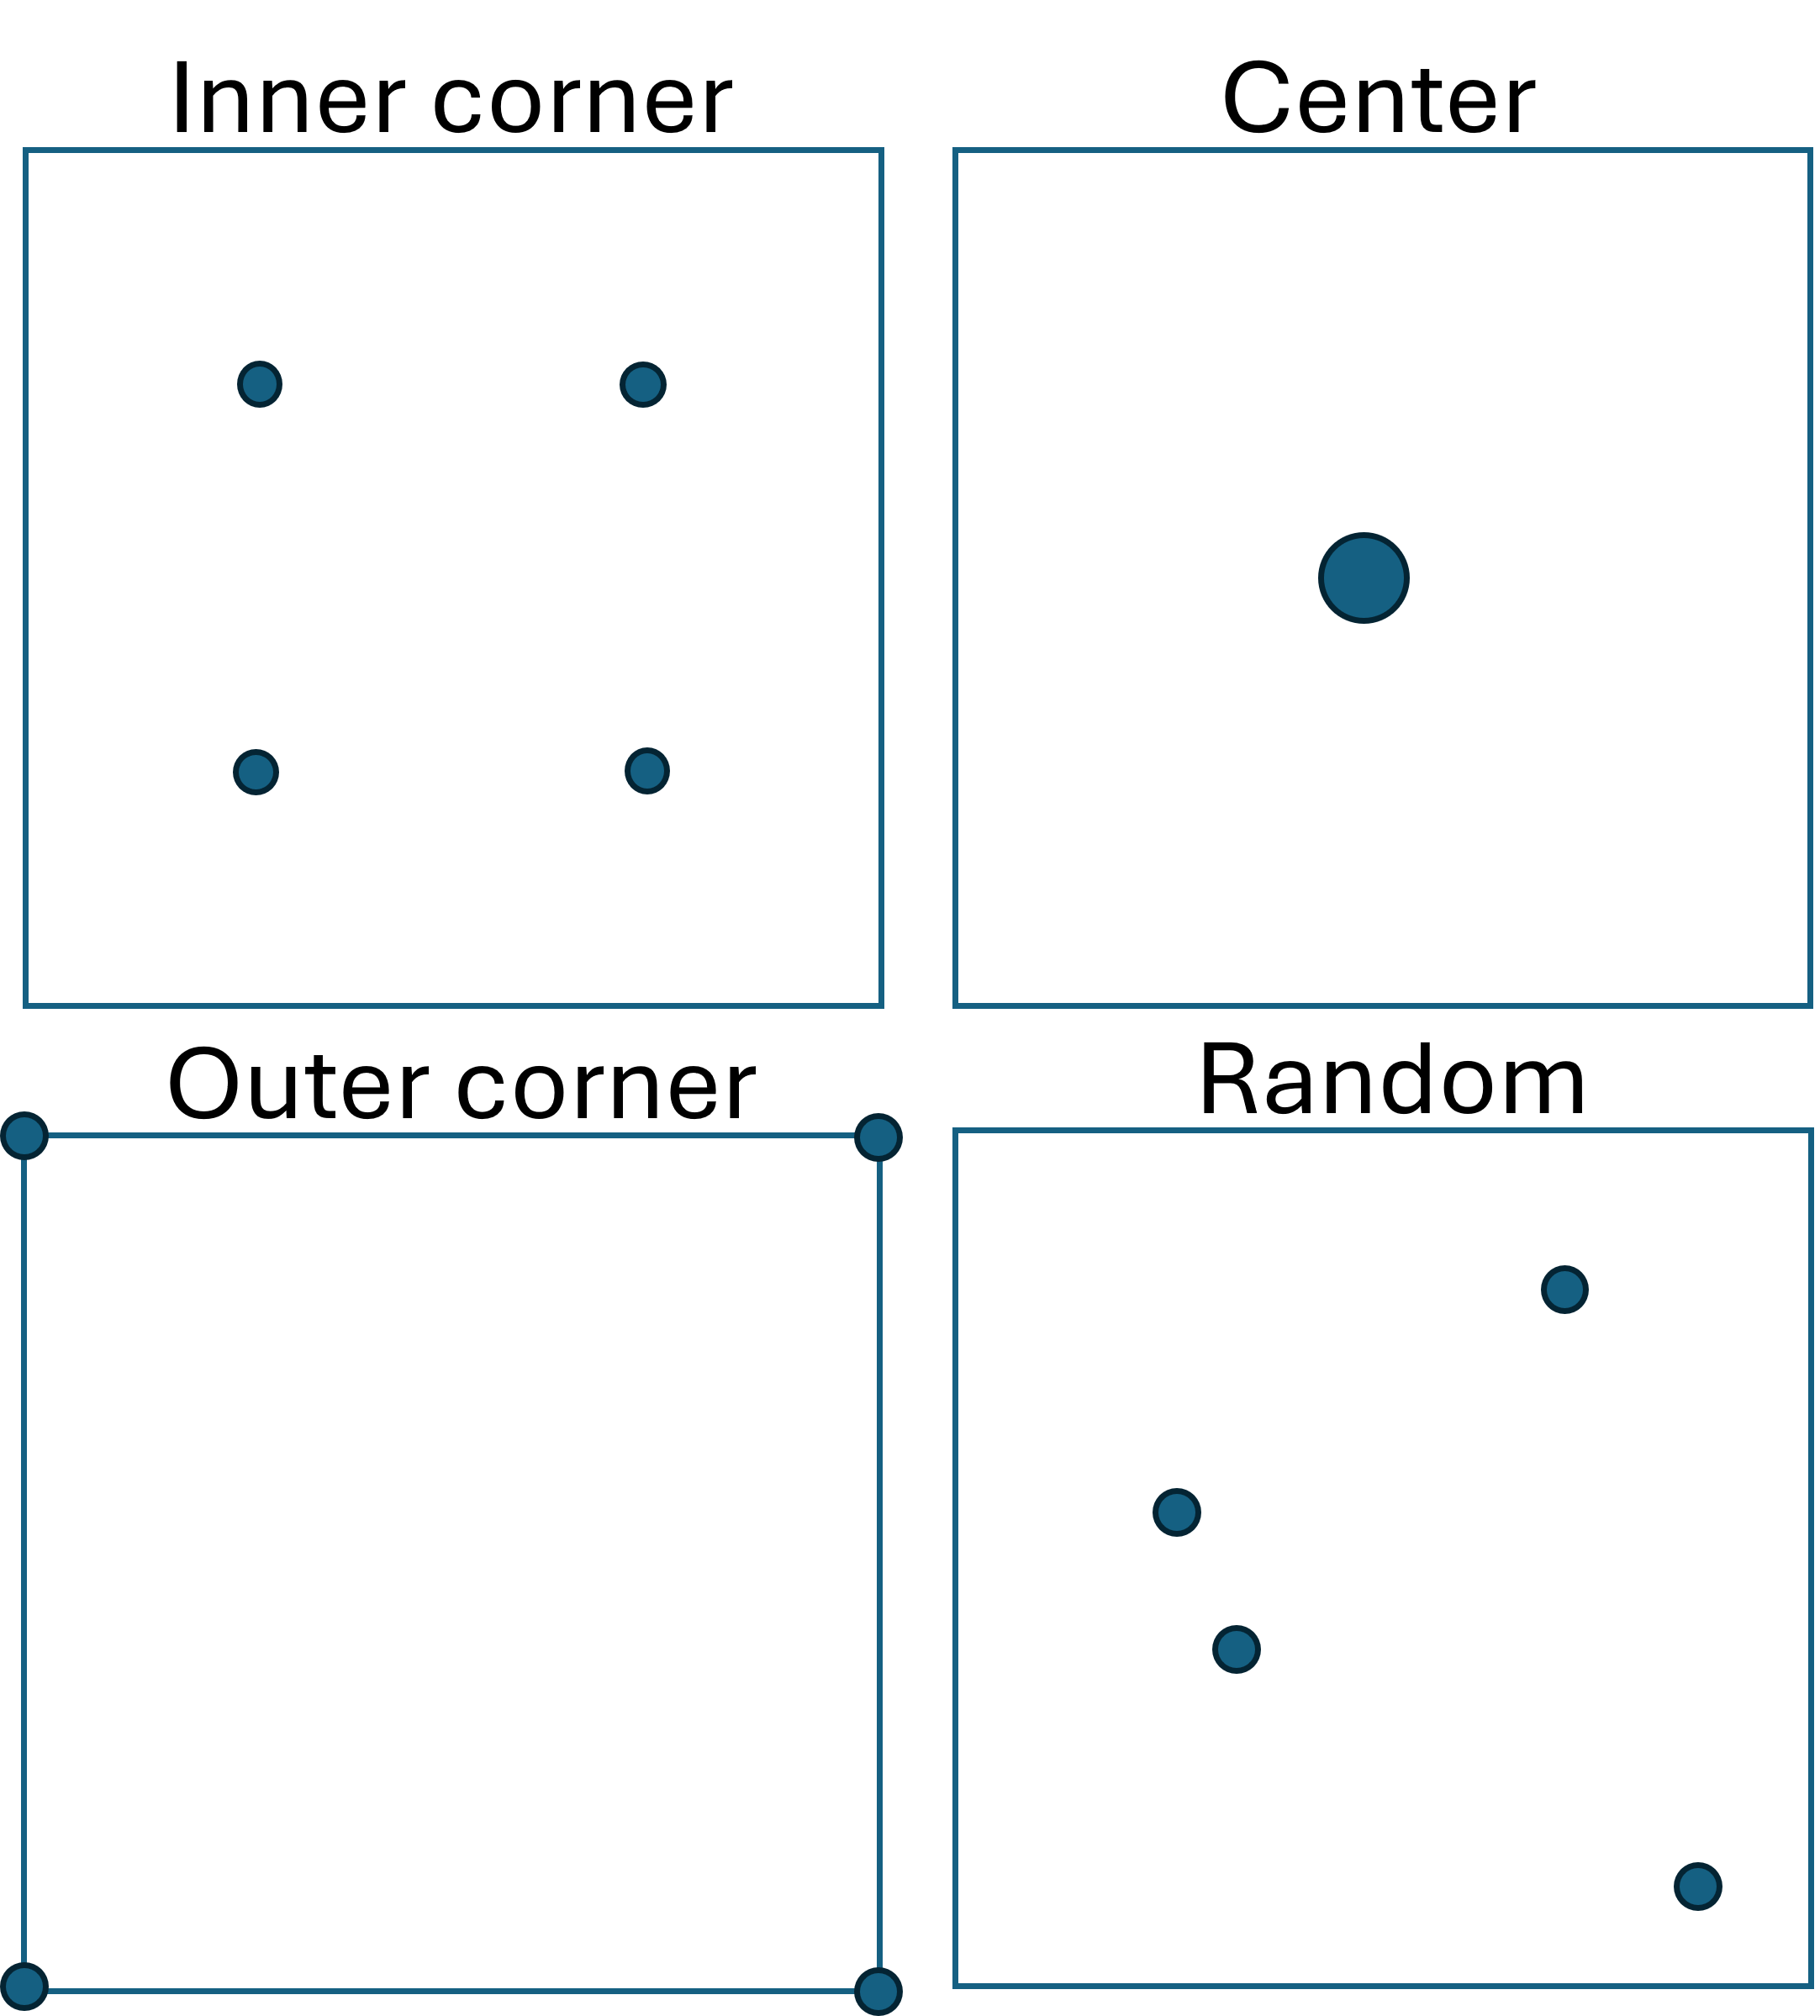
\includegraphics[width=0.50\textwidth]{figs/PI SAs.png}
    \caption{
    Seating arrangements (SAs) considered for the nearest-neighbor (PI) regime.
    Dots represent the initial positions of learned agents ($s_{i,j}=1$) in the lattice.
    Agents are otherwise arranged in a rectangular lattice pattern (shown here as square for brevity).
    The random case shown is one of many possible arrangements.
    }
    \label{fig:PI-SAs}
\end{figure}
Four arrangements are considered: inner corner, outer corner, center, and random, following prior work on the role of seating in classroom learning~\citep{roxas2010seating, monterola2009}.
Unless otherwise specified, the inner corner arrangement is used as the default for the nearest-neighbor regime in the results that follow.

\section{Results and Discussion}\label{sec:rnd}

The following results characterize the collective relaxation dynamics of the pCA model under both interaction regimes across a range of system sizes $N$, coupling strengths $\rho_0$, and heterogeneity levels $\delta\lambda$.
All quantities presented are averages over twenty independent randomized runs, with bands in all plots representing the min-max range across runs.

\subsection{Relaxation dynamics: broadcast versus nearest-neighbor regimes}

  The two regimes exhibit qualitatively distinct relaxation dynamics, as shown in Fig.~\ref{fig:comparison size}.
  In the broadcast regime, the global coupling mechanism drives a rapid early onset of transitions across the entire agent population simultaneously, with the relaxation rate tapering off in the later stages as agents with lower $\lambda$ values transition more slowly.
  In the nearest-neighbor regime, the spread of the learned state is governed by a percolation-like process, producing a gradual initial increase in the learned fraction followed by a sharp rise as the number of active learned-unlearned interfaces grows.
  The nearest-neighbor regime catches up to and surpasses the broadcast regime in the later stages of relaxation, particularly for small $N$, and this observation holds consistently across all seating arrangements considered.
  This two-stage relaxation behavior --- an early broadcast-driven stage followed by a percolation-driven surge --- becomes particularly pronounced under high heterogeneity, as discussed in the following subsection.

  \begin{figure}[htbp]
    \centering
    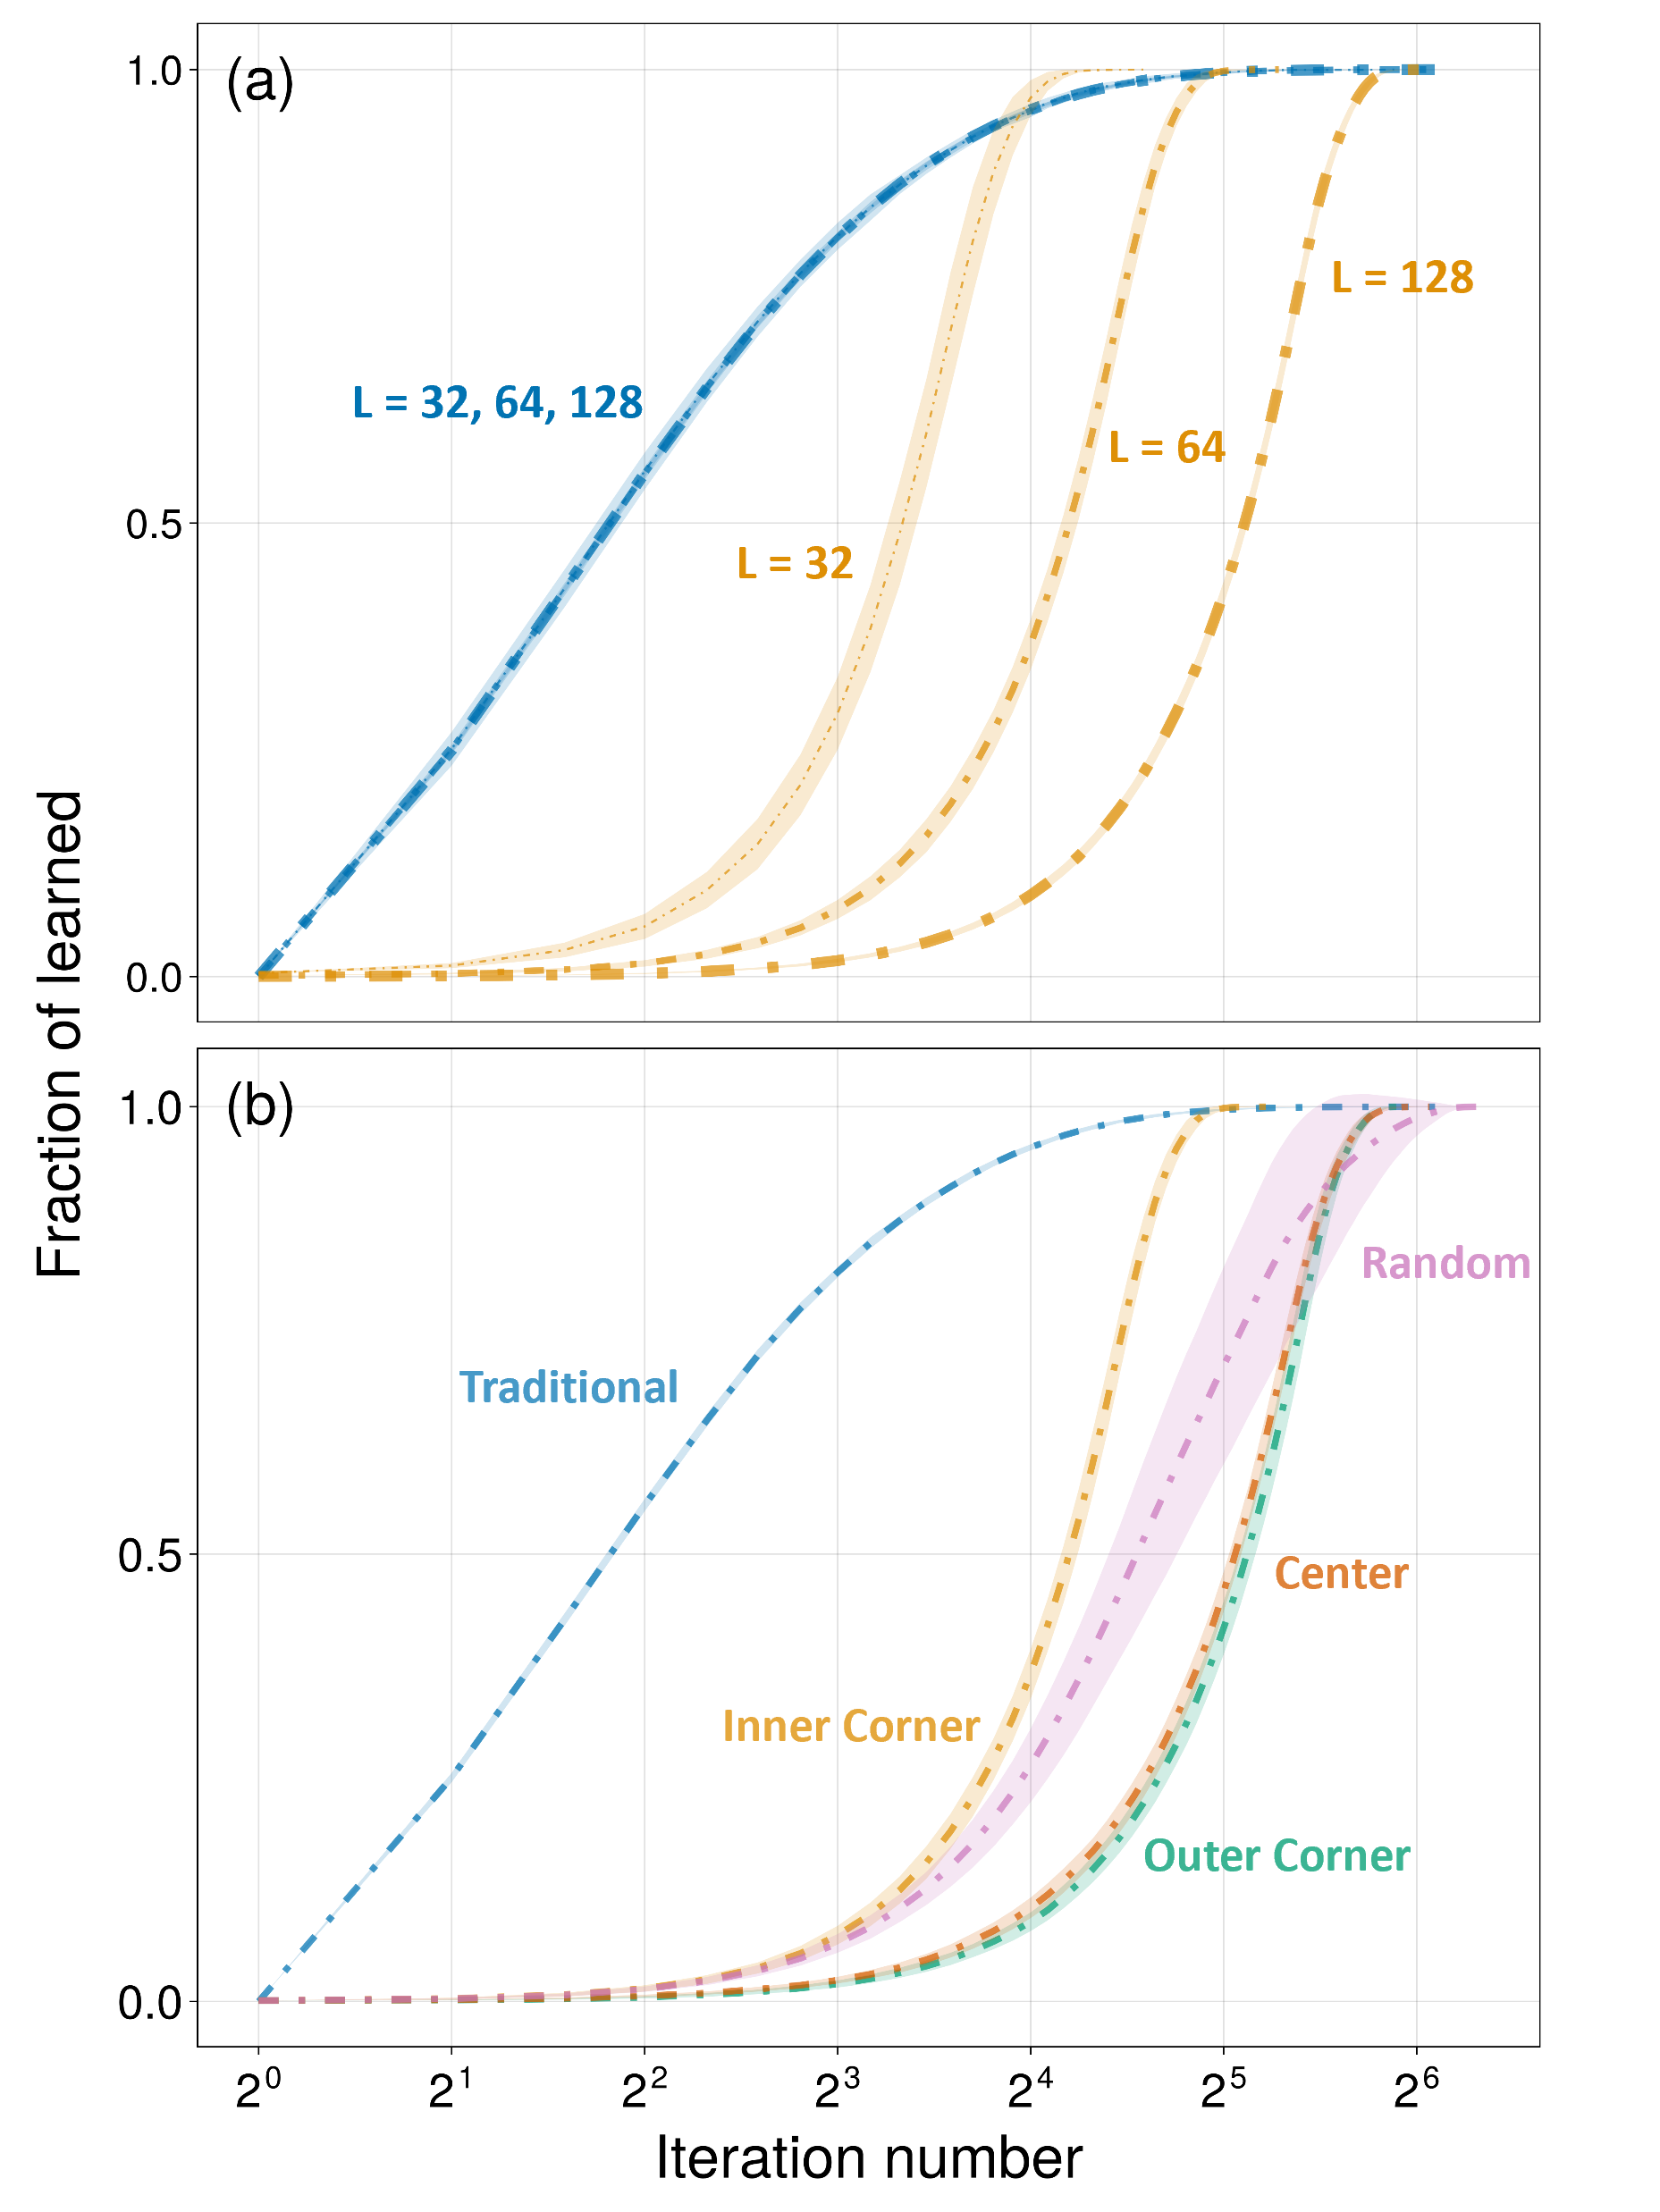
\includegraphics[width=0.60\textwidth]{figs/figure-3.png}
    \caption{
    Monotonic increase of the learned agent fraction over iteration number for both interaction regimes.
    Blue corresponds to the broadcast (TI) regime; all other colors correspond to the nearest-neighbor (PI) regime with different seating arrangements (SAs): yellow-orange (inner corner), orange (center), green (outer corner), and pink (random).
    Line width is proportional to system size $N$.
    Bands represent the min-max range across $20$ independent randomized runs.
    Fixed parameters: $\rho_0=0.5$, $\delta\!\lambda=0.2$.
    (a)~Effect of system size $N$; the inner corner SA is used for the nearest-neighbor regime.
    (b)~Effect of seating arrangement for a fixed system size.
    }
    \label{fig:comparison size}
  \end{figure}

  Fig.~\ref{fig:comparison size}(a) shows the effect of system size $N$ on the relaxation curves.
  The broadcast regime is largely unaffected by system size, as expected from the global coupling mechanism in which each agent updates independently of its neighbors.
  In the nearest-neighbor regime, increasing $N$ delays the onset of the sharp rise in the learned fraction without significantly affecting the slope of that rise, resulting in a shift of $t_{\rm max}$ with system size while the overall curve shape is preserved.

  Fig.~\ref{fig:comparison size}(b) shows the effect of seating arrangement on the nearest-neighbor regime.
  The inner corner arrangement produces the earliest onset of the sharp rise, outperforming all other arrangements considered.
  Similarly to the effect of system size, different seating arrangements primarily shift the onset of the sharp rise rather than its slope --- with the exception of the random arrangement, which affects both the slope of the rise and exhibits the widest min-max band across runs.
  The center and outer corner arrangements perform similarly, a consequence of the isotropic coupling assumption in the model.

\subsection{Effects of coupling strength and agent heterogeneity}

    The coupling strength $\rho_0$ and heterogeneity parameter $\delta\lambda$ are the two key parameters governing the relaxation dynamics, and their effects are shown in Fig.~\ref{fig:comparison rates}.

    As shown in Fig.~\ref{fig:comparison rates}(a), increasing $\rho_0$ shifts the relaxation curve earlier along the iteration axis for both regimes, reflecting the higher per-step probability of transitioning to the learned state.
    This shift is nonlinear --- a change from $\rho_0=0.1$ to $0.5$ produces a larger shift than the same increment from $\rho_0=0.5$ to $0.9$.
    The broadcast regime shows an earlier onset of learning for all values of $\rho_0$, consistent with its global coupling mechanism.
    The nearest-neighbor regime, by contrast, exhibits a more stable curve shape across varying $\rho_0$, with coupling strength introducing primarily a delay in onset rather than a change in the character of the relaxation.

    The effect of agent heterogeneity $\delta\lambda$ is shown in Fig.~\ref{fig:comparison rates}(b) and reveals a qualitative difference between the two regimes.
    In the broadcast regime, increasing $\delta\lambda$ introduces a pronounced two-stage relaxation: a fast initial stage driven by the high-$\lambda$ subpopulation, followed by a slow residual stage as the low-$\lambda$ subpopulation transitions on a longer timescale.
    This two-stage behavior becomes most pronounced at $\delta\lambda=0.45$, where the separation between the two relaxation stages is most clearly visible.
    At the extreme value of $\delta\lambda=0.49$ --- corresponding to subpopulations with $\lambda=0.01$ and $\lambda=0.99$ --- an unexpected four-stage relaxation process is observed in the broadcast regime, alternating between fast and slow relaxation stages.
    While the underlying mechanism for this behavior is not fully understood within the present model, we note that this parameter regime is far outside any realistic range and report it here as a suggestive result warranting further investigation.
    In the nearest-neighbor regime, heterogeneity produces only a gradual uniform delay in the relaxation curve across all values of $\delta\lambda$ considered, with no qualitative change in curve shape --- the percolation-driven spreading process effectively averages over the heterogeneous $\lambda$ distribution as the learned state propagates through the lattice.

    The spatial evolution of the learned state across the lattice provides further insight into these dynamical differences, as shown in Fig.~\ref{fig:comparison rates}(c) for a smaller system size $N=32$ for visual clarity.
    In the broadcast regime, agents with high $\lambda$ values transition first, appearing as isolated learned sites distributed across the lattice, with low-$\lambda$ agents filling in slowly afterward.
    In the nearest-neighbor regime, the learned state spreads outward from the initial seed sites as a connected front, with the percolation-like propagation producing the characteristic sharp rise in the learned fraction observed in the relaxation curves.
    These observations suggest that a combination of both regimes --- an initial broadcast phase to seed learned agents across the lattice, followed by a nearest-neighbor phase to propagate learning through percolation --- would harness the advantages of both dynamics, consistent with current instructional practices~\citep{mazur1997peer, smith2009peer, lasry2008peer, roxas2010seating}.

    \begin{figure}[htbp]
        \centering
        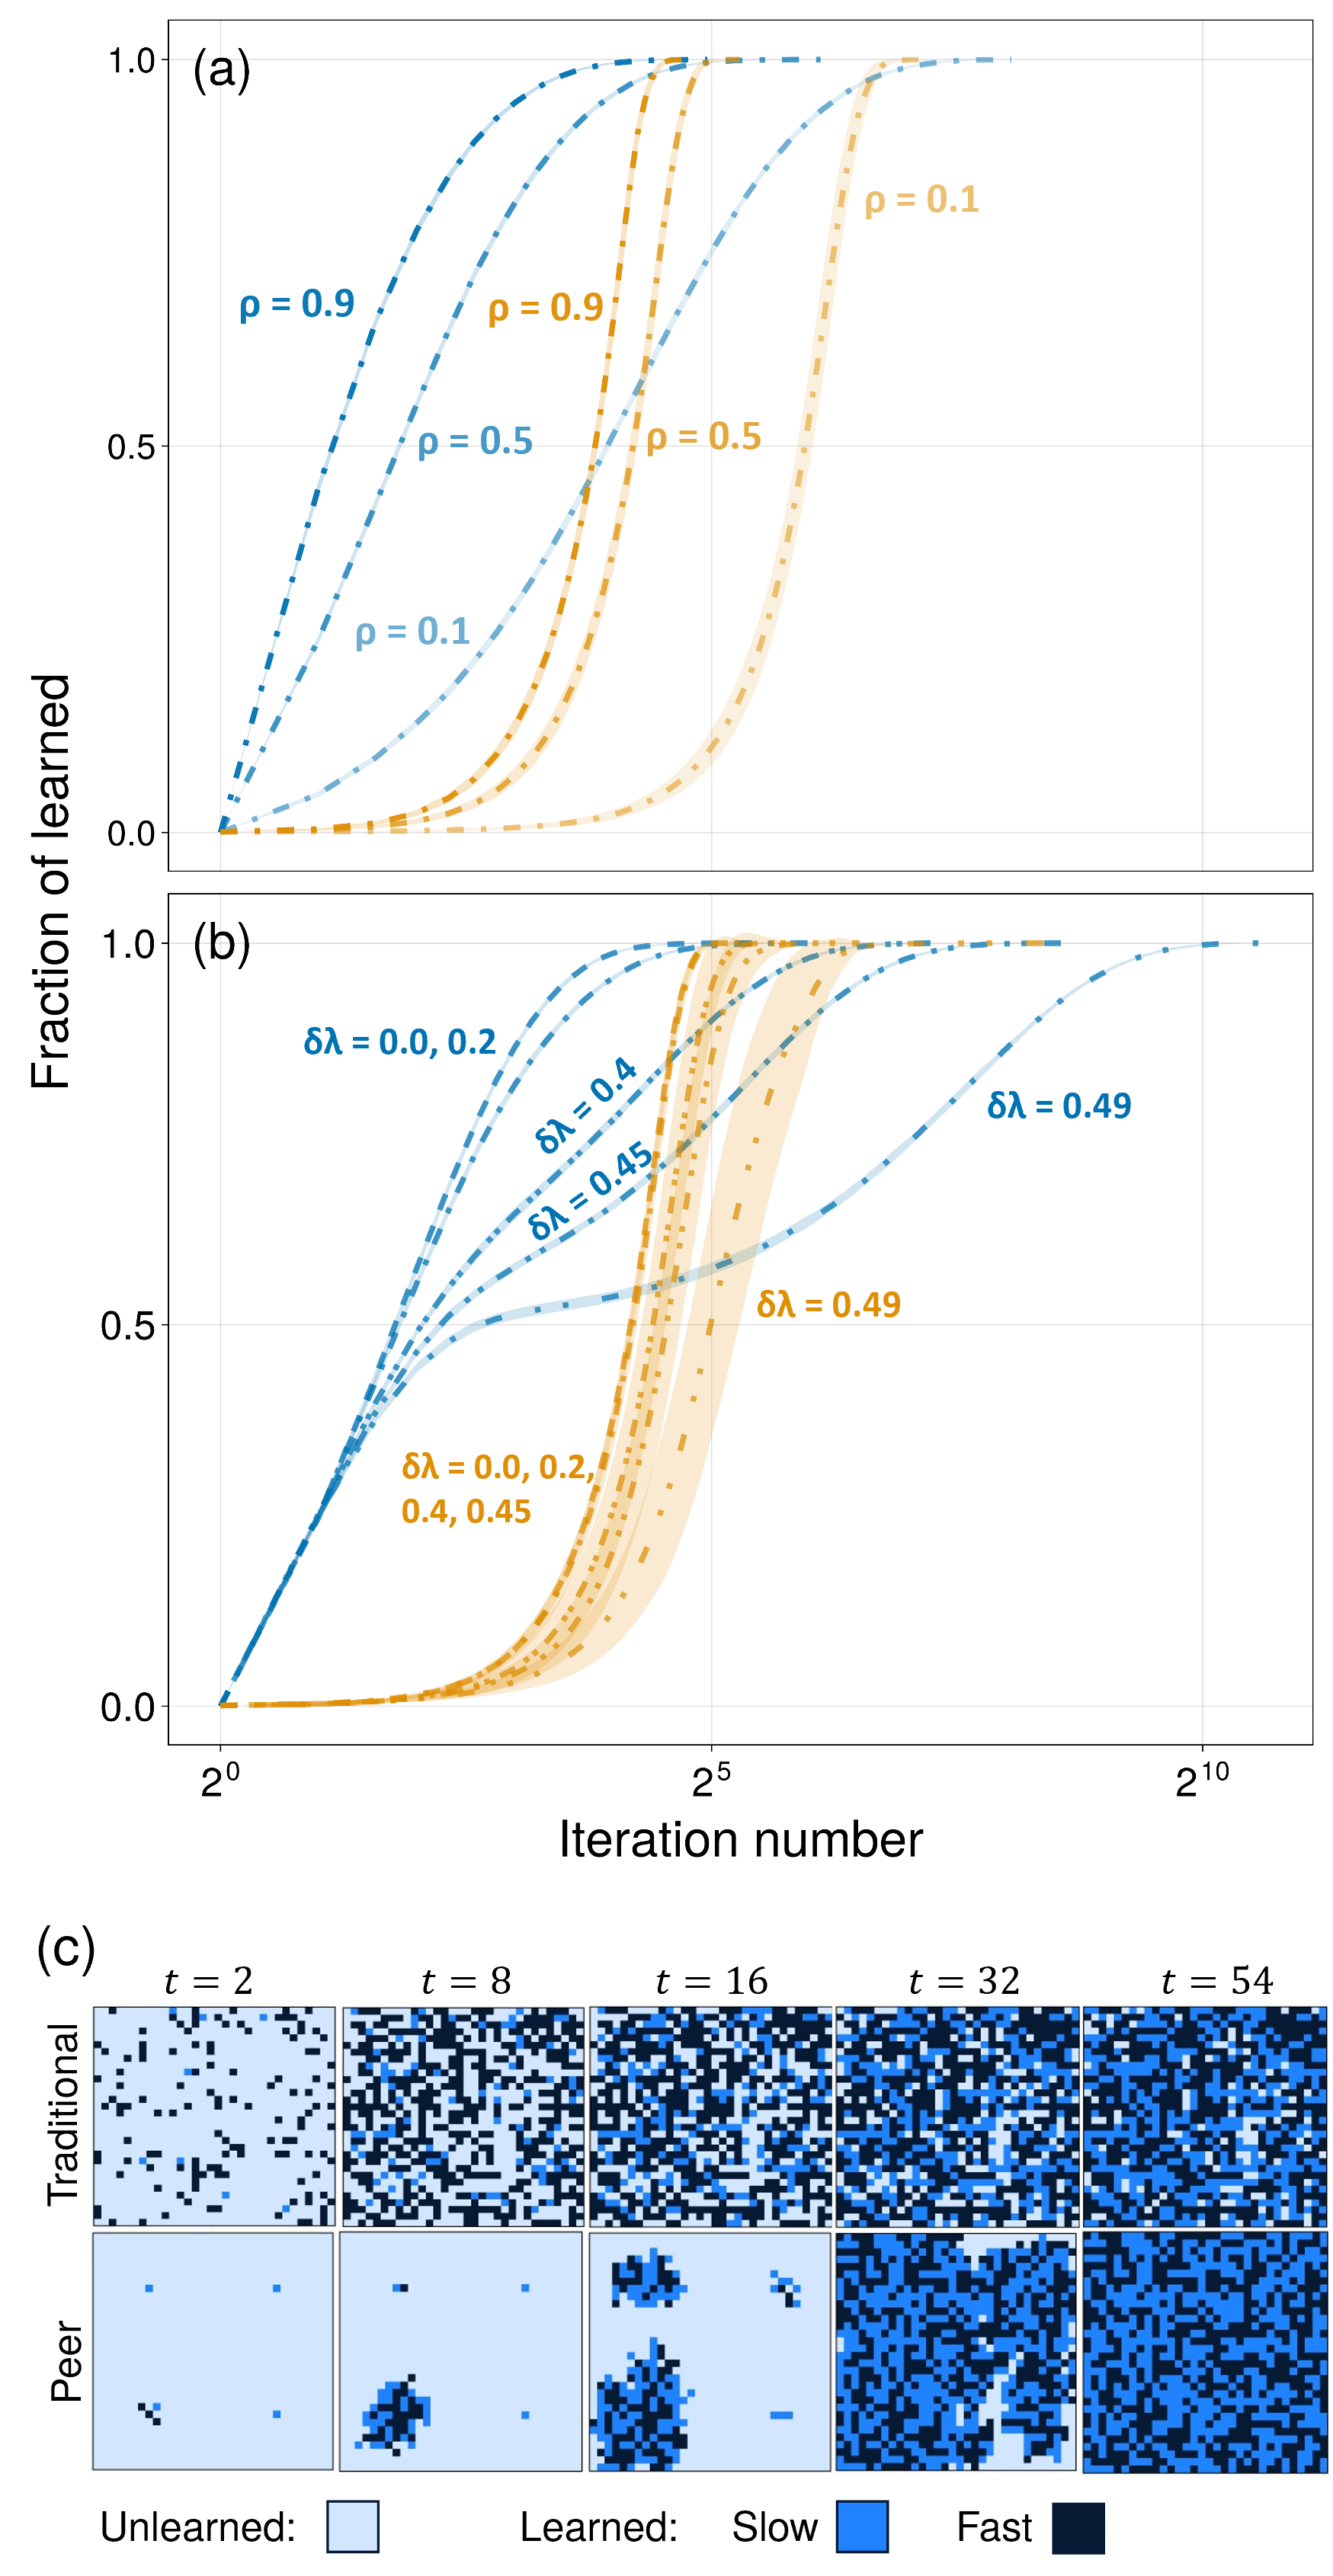
\includegraphics[width=0.5\textwidth]{figs/figure4.png}
        \caption{
        Monotonic increase of the learned agent fraction over iteration number for both interaction regimes.
        Blue lines represent the broadcast (TI) regime and orange lines represent the nearest-neighbor (PI) regime with inner corner seating arrangement.
        Bands represent the min-max range across $20$ independent randomized runs.
        Fixed parameters unless otherwise indicated: $N=64$, $\rho_0=0.5$, $\delta\lambda=0.2$, inner corner SA for the nearest-neighbor regime.
        (a)~Effect of coupling strength $\rho_0$.
        (b)~Effect of heterogeneity parameter $\delta\lambda$.
        (c)~Representative spatial configurations of the lattice ($L=32$, $\rho_0=0.3$) at successive iteration numbers (each column doubles the previous $t$, starting from $t=2$) for the broadcast regime (top row) and nearest-neighbor regime (bottom row).
        Color intensity encodes agent learning rate, with darker shades indicating higher $\lambda$ values.
        }
        \label{fig:comparison rates}
    \end{figure}

\subsection{Combined effects of coupling strength and heterogeneity}

    The combined effects of coupling strength $\rho_0$ and heterogeneity $\delta\lambda$ on the total relaxation time $t_{\rm max}$ are summarized in Fig.~\ref{fig:Params effect summary t} for two system sizes, $N=32^2$ and $N=128^2$.
    Higher $t_{\rm max}$ is disadvantageous, corresponding to slower collective relaxation of the agent population.

    For small system sizes (Fig.~\ref{fig:Params effect summary t}(a)), the nearest-neighbor regime consistently outperforms the broadcast regime at high $\delta\lambda$, with the performance gap increasing significantly as heterogeneity increases.
    This advantage diminishes at higher $\rho_0$, where the broadcast regime benefits more strongly from increased coupling strength.
    For large system sizes (Fig.~\ref{fig:Params effect summary t}(b)), this relationship can reverse for low heterogeneity and high coupling strength, where the broadcast regime produces shorter $t_{\rm max}$ than the nearest-neighbor regime.

    Notably, the performance difference is strongly asymmetric: when the broadcast regime outperforms the nearest-neighbor regime, the difference in $t_{\rm max}$ is relatively small, whereas when the nearest-neighbor regime outperforms the broadcast regime, the difference can be very large.
    This asymmetry suggests that the nearest-neighbor regime is a relatively safe choice --- it never performs drastically worse than the broadcast regime, but can perform substantially better under heterogeneous conditions.
    A combination of both regimes would therefore be optimal, exploiting the fast early-stage relaxation of the broadcast regime and the robustness of the nearest-neighbor regime under heterogeneity.

    \begin{figure}[htbp]
        \centering
        
\includegraphics[width=0.60\textwidth]{figs/figure5.png}
        \caption{
        Total relaxation time $t_{\rm max}$ as a function of coupling strength $\rho_0$ and heterogeneity $\delta\lambda$ for the broadcast (blue surface) and nearest-neighbor (orange surface) regimes, for two system sizes:
        (a)~$N=32^2$ and (b)~$N=128^2$.
        The nearest-neighbor regime uses the inner corner seating arrangement.
        Lower $t_{\rm max}$ indicates faster collective relaxation.
        }
        \label{fig:Params effect summary t}
    \end{figure}

\subsection{Comparison with empirical data and theoretical predictions}

    The return map --- a plot of the learned fraction at iteration $t$ against that at iteration $t-1$ --- provides a means of characterizing the fixed-point structure of the relaxation dynamics and connecting simulation results to empirical classroom data.
    Following the mapping $S \rightarrow f$, where $f$ is the fraction of learned agents, the Hake gain $g$ can be approximated from simulation or empirical data via
    %%
    \begin{equation}\label{eq:gain-from-return-map}
    g(f) = \frac{h(f) - f}{1 - f}
    \end{equation}
    %%
    where $h(f)$ is a fitting function to the return map data following the recurrence relation $f_t = h(f_{t-1})$.

    Fig.~\ref{fig:Return map} shows the return maps obtained from simulation data for both regimes across selected parameter sets, alongside empirical classroom data provided by Roxas (co-author).
    The broadcast regime consistently produces a linear return map, well described by
    %%
    \begin{equation}
        h(f) = a_0 + (1-a_0)f \;{\rm [broadcast]}
    \end{equation}
    %%
    corresponding to a constant Hake gain $g(f) = m$, where $m$ replaces $a_0$ for distinction.\footnote{Large $N$: $f_t = 0.97 f_{t-1} + 0.029$; small $N$: $f_t = 0.548 f_{t-1} + 0.452$.}
    The nearest-neighbor regime, by contrast, produces a quadratic return map
    %%
    \begin{equation}
        h(f) = a_0 + [1-(a_0+a_2)]f + a_2f^2 \;{\rm [nearest\text{-}neighbor]}
    \end{equation}
    %%
    corresponding to a linear Hake gain $g(f) = a_0 - a_2 f$, consistent with the theoretical prediction of~\citet{nitta2019mathematical} in the limit $a_0 \approx 0$.\footnote{Large $N$: $f_t = -0.033 f^2_{t-1} + 1.033 f_{t-1}$; small $N$: $f_t = -0.605 f^2_{t-1} + 1.595 f_{t-1} + 0.019$.}

    The magnitude of $|a_2|$ serves as a measure of the efficiency of the nearest-neighbor regime, decreasing from $|a_2|=0.60$ for $N=32^2$ to $|a_2|=0.03$ for $N=128^2$, reflecting the loss of nearest-neighbor efficiency with increasing system size.
    The broadcast regime gain similarly declines from $m=0.45$ to $m=0.029$ over the same range, consistent with the $t_{\rm max}$ results presented above.

    The empirical dataset, consisting of pre- and post-test scores from fourteen classrooms, spans a broad range of values and exhibits considerable scatter, reflecting the many factors influencing real classroom dynamics.
    A quadratic fit to this data yields $a_2=0.14$, falling between our favorable ($a_2=-0.605$) and unfavorable ($a_2=-0.033$) simulation cases, though the fit quality is limited by the variance in the data.\footnote{Roxas' data: $f_t = 0.14 f_{t-1}^2 + 0.68 f_{t-1} + 0.13$.}
    The sign difference between the empirical and simulation quadratic coefficients is notable --- the empirical data yields a positive $a_2$ while our nearest-neighbor simulations yield negative $a_2$ --- and may reflect the influence of factors not captured in our model, including mixed instructional strategies, assessment timing, and the presence of score decreases from pre- to post-test, which our binary-state model does not reproduce.

    A discrepancy also exists between our seating arrangement results and those of Roxas~\citep{roxas2010seating}: our model finds the inner corner arrangement to be optimal, while Roxas' empirical results favor the outer corner.
    This difference is attributable to simplifications in our model --- specifically the isotropic coupling assumption and the absence of aptitude similarity effects, whereby agents of similar aptitude learn more effectively when grouped together regardless of their absolute aptitude level~\citep{smith2009peer}.
    These effects are more naturally captured by a continuous-state model and represent a direction for future development.

    Taken together, these results indicate that while our model does not reproduce all features of empirical classroom data, the return map approach provides a tractable framework for characterizing the fixed-point structure of the learning dynamics and extracting class-level Hake gains from pre- and post-test data.

    \begin{figure}[htbp]
        \centering
        
\includegraphics[width=0.60\textwidth]{figs/figure6.png}
        \caption{
        Return map of the learned agent fraction $f_t$ against $f_{t-1}$ for selected parameter sets.
        Blue circles represent broadcast (TI) regime data points; orange squares represent nearest-neighbor (PI) regime data points; pink diamonds represent empirical data from Roxas (co-author).
        Darker points indicate higher overlap of data points at those coordinates.
        Dashed lines show the best-fit functions obtained using the Levenberg-Marquardt algorithm for each dataset.
        The green line represents the theoretical prediction of~\citet{nitta2019mathematical} and the gray line represents $y=x$.
        (a)~Large system size $N=128^2$.
        (b)~Small system size $N=32^2$.
        }
        \label{fig:Return map}
    \end{figure}

\section{Summary and Conclusion}

We have presented a probabilistic cellular automata (pCA) model for investigating the collective relaxation dynamics of a heterogeneous agent population under two distinct interaction topologies: a broadcast regime, analogous to traditional instruction, and a nearest-neighbor regime, analogous to peer instruction.
The model is defined on a two-dimensional rectangular lattice, with each agent assigned a binary state and an individual learning rate $\lambda$ drawn from a two-level heterogeneous distribution parameterized by $\delta\lambda$.

The two regimes exhibit qualitatively distinct relaxation dynamics.
The broadcast regime drives a rapid early onset of transitions across the agent population, but is sensitive to agent heterogeneity --- high $\delta\lambda$ produces a pronounced two-stage relaxation, with the fast initial stage driven by the high-$\lambda$ subpopulation and the slow residual stage governed by the low-$\lambda$ subpopulation.
The nearest-neighbor regime exhibits percolation-driven spreading dynamics, producing a gradual initial increase in the learned fraction followed by a sharp rise as the number of active interfaces grows.
This regime is more robust to agent heterogeneity, exhibiting only a uniform delay in the relaxation curve across all $\delta\lambda$ values considered, with no qualitative change in curve shape.

The combined effects of $\rho_0$ and $\delta\lambda$ on the total relaxation time $t_{\rm max}$ reveal an asymmetric performance relationship between the two regimes.
The broadcast regime is favored for large system sizes and low heterogeneity, while the nearest-neighbor regime is favored for small system sizes and high heterogeneity.
The performance gap is notably larger in the latter case, suggesting that the nearest-neighbor regime is a relatively safe choice --- never performing drastically worse than the broadcast regime, but capable of performing substantially better under heterogeneous conditions.
A combination of both regimes is therefore expected to be optimal, exploiting the fast early-stage relaxation of the broadcast regime and the robustness of the nearest-neighbor regime under heterogeneity.

The fixed-point structure of the relaxation dynamics was further characterized through a return map analysis, from which class-level Hake gains were extracted analytically.
The broadcast regime yields a constant gain $g(f)=m$, while the nearest-neighbor regime yields a linear gain $g(f)=a_0-a_2f$, consistent with existing theoretical predictions~\citep{nitta2019mathematical}.
The return map approach was also applied to empirical classroom data, showing qualitative agreement despite the scatter in the data, and we propose it as a practical method for empirically estimating class-level Hake gains from pre- and post-test results.

While the present model is necessarily simplified, it captures the essential dynamical features of both interaction regimes and provides a tractable framework for investigating the effects of system size, coupling strength, and agent heterogeneity on collective relaxation dynamics.
Future extensions of the model could incorporate continuous-valued agent states to capture aptitude similarity effects, anisotropic coupling to account for spatial orientation in the classroom, and a mixed-regime model that explicitly combines broadcast and nearest-neighbor phases within a single simulation.

% Numbered list
% Use the style of numbering in square brackets.
% If nothing is used, default style will be taken.
%\begin{enumerate}[a)]
%\item 
%\item 
%\item 
%\end{enumerate}  

% Unnumbered list
%\begin{itemize}
%\item 
%\item 
%\item 
%\end{itemize}  

% Description list
%\begin{description}
%\item[]
%\item[] 
%\item[] 
%\end{description}  

% \clearpage %%Remove this from your manuscript


% % Figure
% \begin{figure}%[]
%   \centering
% %    \includegraphics{}
%     \caption{}\label{fig1}
% \end{figure}


% \begin{table}%[]
% \caption{}\label{tbl1}
% \begin{tabular*}{\tblwidth}{@{}LL@{}}
% \toprule
%   &  \\ % Table header row
% \midrule
%  & \\
%  & \\
%  & \\
%  & \\
% \bottomrule
% \end{tabular*}
% \end{table}

% Uncomment and use as the case may be
%\begin{theorem} 
%\end{theorem}

% Uncomment and use as the case may be
%\begin{lemma} 
%\end{lemma}

%% The Appendices part is started with the command \appendix;
%% appendix sections are then done as normal sections
%% \appendix

% \section{}\label{}

% To print the credit authorship contribution details
\printcredits

%% Loading bibliography style file
%\bibliographystyle{model1-num-names}
\bibliographystyle{cas-model2-names}

% Loading bibliography database
\bibliography{cas-refs}

% Biography
%\bio{}
% Here goes the biography details.
%\endbio

%\bio{pic1}
% Here goes the biography details.
%\endbio

\end{document}

